% \chapter{Validation expérimentale de RevMine}

% \label{chap:validation-experimentale}

\section{Introduction}
\label{sec:validation-introduction}

La validation de RevMine doit démontrer trois propriétés complémentaires. Premièrement, la
plateforme doit fonctionner sans régression sur ses principaux parcours techniques. Deuxièmement,
les données collectées depuis GitHub et GitLab doivent être complètes, exactes et comparables à
une vérité terrain indépendante. Troisièmement, les métriques et visualisations produites doivent
être conformes à leurs définitions mathématiques.

Ce chapitre commence donc par les résultats de tests automatisés, l'analyse statique et la
couverture de code. Il présente ensuite une démarche statistique de validation, puis l'applique à
la collecte, aux calculs analytiques, aux visualisations, à la reproductibilité et à la couche
d'orchestration LLM. L'axe méthodologique central reste la \textbf{validation différentielle par
oracle indépendant}~: les résultats produits par RevMine sont comparés à un calcul de référence
réalisé à partir des mêmes données brutes, sans réutiliser les fonctions internes de RevMine. Cette
approche suit les principes de validation des métriques logicielles, selon lesquels une mesure doit
être définie explicitement, calculée selon un protocole stable et vérifiée par rapport à l'attribut
qu'elle prétend mesurer \cite{fenton2014software,kitchenham1995framework}. La structuration des
objectifs suit également l'approche Goal--Question--Metric, qui relie chaque objectif à des
questions observables et à des métriques mesurables \cite{basili1994gqm}.

\section{Résultats des tests automatisés}
\label{sec:resultats-tests-automatises}

\subsection{Exécution des suites de tests}

Les rapports JUnit générés pour les six services Python totalisent \textbf{561~tests exécutés},
avec \textbf{0 échec}, \textbf{0 erreur} et \textbf{0 test ignoré}. En complément, les tests
unitaires frontend exécutés avec Jest totalisent \textbf{29~tests réussis} sur trois suites. Les
scénarios Cypress constituent la validation fonctionnelle de bout en bout~; ils sont conservés
comme niveau de validation globale des parcours utilisateur.

\begin{table}[H]
\centering
\small
\caption{Résultats d'exécution des tests automatisés}
\label{tab:resultats-tests-automatises}
\begin{tabular}{|>{\raggedright\arraybackslash}p{4cm}
                |>{\centering\arraybackslash}p{2.2cm}
                |>{\centering\arraybackslash}p{1.8cm}
                |>{\centering\arraybackslash}p{1.8cm}
                |>{\centering\arraybackslash}p{2cm}|}
\hline
\textbf{Service / couche} & \textbf{Outil} & \textbf{Tests} & \textbf{Échecs} & \textbf{Durée} \\
\hline
API Gateway & pytest & 7 & 0 & 2,999~s \\
\hline
Authentification & pytest & 38 & 0 & 11,153~s \\
\hline
Configuration & pytest & 111 & 0 & 3,096~s \\
\hline
Collecte & pytest & 220 & 0 & 4,633~s \\
\hline
Analyse & pytest & 161 & 0 & 37,770~s \\
\hline
Service LLM & pytest & 24 & 0 & 0,435~s \\
\hline
Frontend & Jest & 29 & 0 & 1,615~s \\
\hline
Parcours utilisateur & Cypress & 3 fichiers & à renseigner & à renseigner \\
\hline
\end{tabular}
\end{table}

Le taux de succès des tests automatisés est calculé par la formule suivante, où $N$ est le nombre
total de tests exécutés, $F$ le nombre d'échecs et $E$ le nombre d'erreurs d'exécution~:

\begin{equation}
\mathrm{TestSuccessRate} = \frac{N - F - E}{N}
\end{equation}

Pour les suites backend Python et frontend Jest exécutées, le taux observé est donc de
$100\,\%$. Les scénarios Cypress doivent être reportés avec la même logique après exécution dans
l'environnement complet, car ils valident l'enchaînement réel des écrans et des appels API.

\subsection{Couverture de code}

Le Tableau~\ref{tab:couverture} présente les derniers rapports \texttt{coverage.xml} disponibles
pour les services Python. Ces valeurs correspondent aux rapports bruts produits par pytest avant
l'application des exclusions SonarQube.

\begin{table}[H]
\centering
\small
\caption{Taux de couverture des tests backend Python par service}
\label{tab:couverture}
\begin{tabular}{|>{\raggedright\arraybackslash}p{4.5cm}
                |>{\centering\arraybackslash}p{3.2cm}
                |>{\centering\arraybackslash}p{3.2cm}
                |>{\centering\arraybackslash}p{2.8cm}|}
\hline
\textbf{Service} & \textbf{Lignes valides} & \textbf{Lignes couvertes} & \textbf{Couverture} \\
\hline
API Gateway & 137 & 128 & \textbf{93,43\,\%} \\
\hline
Authentification & 356 & 324 & \textbf{91,01\,\%} \\
\hline
Service de configuration & 687 & 589 & \textbf{85,74\,\%} \\
\hline
Service de collecte & 3\,128 & 2\,525 & \textbf{80,72\,\%} \\
\hline
Service d'analyse & 3\,018 & 2\,117 & \textbf{70,15\,\%} \\
\hline
Service LLM & 418 & 389 & \textbf{93,06\,\%} \\
\hline
\textbf{Total backend Python} & \textbf{7\,744} & \textbf{6\,072} & \textbf{78,41\,\%} \\
\hline
\end{tabular}
\end{table}

La couverture frontend n'est pas consolidée dans ce tableau, car la configuration SonarQube du
projet cible le backend. Les tests Jest valident toutefois les modules critiques actuellement
couverts côté interface~: client HTTP, décodage JWT et fournisseur d'authentification.

\section{Analyse statique et qualité du code}
\label{sec:analyse-statique-qualite}

La Figure~\ref{fig:sonar-dashboard} présente le tableau de bord SonarQube utilisé pour suivre la
qualité du backend. L'analyse ne signale aucune issue ouverte en sécurité, aucune issue ouverte
en fiabilité et aucun \textit{security hotspot}. La maintenabilité est notée A malgré
164~issues ouvertes, principalement classées comme dette technique de maintenabilité. La
couverture consolidée par SonarQube atteint \textbf{83,2\,\%} sur environ 6,4k lignes à couvrir,
et le taux de duplication est limité à \textbf{1,6\,\%}.

\begin{figure}[H]
    \centering
    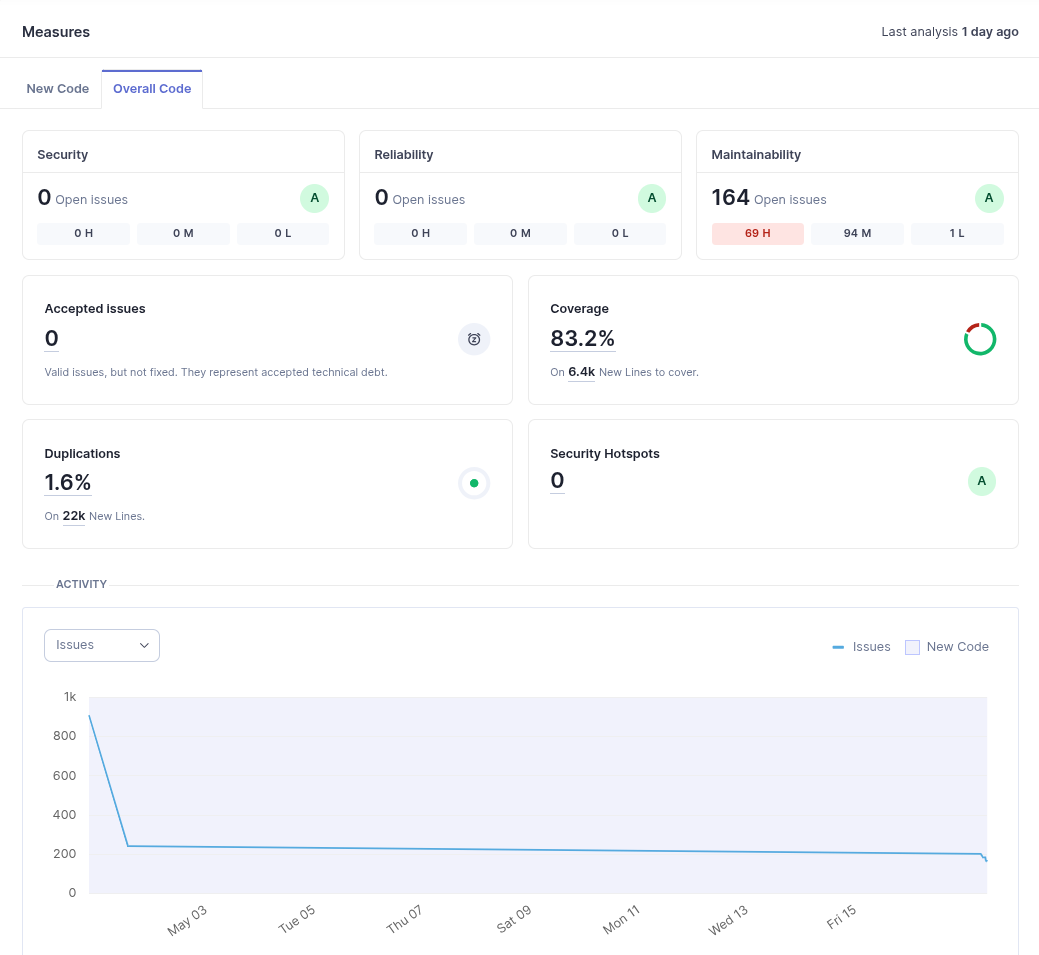
\includegraphics[width=0.95\textwidth]{captures/sonarqube_dashboard.png}
    \caption{Tableau de bord SonarQube -- métriques de qualité de RevMine}
    \label{fig:sonar-dashboard}
\end{figure}

L'écart entre la couverture brute pytest du Tableau~\ref{tab:couverture} et la couverture
SonarQube s'explique par les exclusions définies dans \texttt{sonar-project.properties}. Les
migrations, fichiers de tests, modules de démarrage, adaptateurs techniques et fichiers générés
ne sont pas considérés comme du code métier à couvrir. Cette séparation rend l'indicateur
SonarQube plus représentatif de la logique applicative réellement maintenue.

\section{Démarche de validation statistique}
\label{sec:demarche-validation-statistique}

La validation statistique de RevMine suit une démarche en trois niveaux.

\begin{enumerate}
    \item \textbf{Valider le fonctionnement global}~: vérifier que les tests unitaires,
          d'intégration et end-to-end couvrent les parcours critiques et que leur taux de succès
          est stable.
    \item \textbf{Valider la collecte avec mesure}~: comparer les entités collectées par RevMine
          avec un collecteur de référence indépendant, puis mesurer la complétude, l'exactitude et
          la cohérence multi-plateformes.
    \item \textbf{Valider l'analyse}~: comparer les métriques et séries produites par RevMine
          avec un oracle indépendant, en utilisant des mesures d'écart telles que MAE, RMSE, MAPE,
          EMR et biais moyen.
\end{enumerate}

Le Tableau~\ref{tab:questions-validation-revmine} relie ces niveaux aux questions de validation
et aux indicateurs à renseigner.

\begin{table}[H]
\centering
\small
\caption{Objectifs, questions et indicateurs de validation de RevMine}
\label{tab:questions-validation-revmine}
\begin{tabularx}{\textwidth}{|p{1.4cm}|X|X|X|}
\hline
\textbf{ID} & \textbf{Question de validation} & \textbf{Risque contrôlé} & \textbf{Indicateurs principaux} \\
\hline
QV1 & RevMine exécute-t-il correctement ses parcours techniques critiques ? & Régression fonctionnelle, route cassée, erreur d'orchestration & taux de succès des tests, réussite Cypress, erreurs applicatives \\
\hline
QV2 & RevMine collecte-t-il les entités attendues depuis GitHub et GitLab ? & Données absentes, pagination incomplète, erreur d'API ou de normalisation & FCR, FAR, CPC, taux d'erreur de champs \\
\hline
QV3 & Les métriques calculées par RevMine sont-elles conformes à leurs définitions ? & métriques temporelles, collaboratives ou de code incorrectes & EMR, MAE, RMSE, MAPE, corrélation, biais moyen \\
\hline
QV4 & Les analyses et visualisations reposent-elles sur les bonnes séries numériques ? & graphique correct visuellement mais fondé sur une agrégation erronée & exactitude des séries, distance d'agrégation, erreur relative par point \\
\hline
QV5 & Les résultats sont-ils reproductibles à paramètres constants ? & résultats différents entre deux exécutions identiques & hash des CSV normalisés, écart-type inter-exécutions, coefficient de variation \\
\hline
QV6 & La couche LLM produit-elle des plans structurés conformes au schéma RevMine ? & mauvaise intention, métriques ou dépendances manquantes & validité JSON, exact match, précision, rappel, F1, FDSR \\
\hline
\end{tabularx}
\end{table}

Les sections suivantes détaillent l'application de cette démarche à la collecte, aux métriques,
aux visualisations, à la performance, à la reproductibilité et à l'orchestration LLM.

% ============================================================
\section{Validation de la collecte de données}
\label{sec:validation-collecte}
% ============================================================

\subsection{Protocole expérimental}

La validation de la couche de collecte vise à établir l'exactitude et la complétude des données
produites par RevMine par rapport à une vérité terrain obtenue directement via les API officielles
GitHub et GitLab. Pour éviter que la vérité terrain ne soit conçue pour favoriser RevMine, le
collecteur de référence a été dérivé de la littérature existante. Un inventaire des champs et
des endpoints récupérés par des outils d'extraction établis
\parencite{gousios2017mining, bouraffa2025not, rebatchi2024dependabot, legault2022empirical,
kansab2025empirical} a permis d'implémenter un collecteur de référence récupérant l'union de
leurs surfaces de données directement depuis l'API GitHub REST (v2022-11-28) et l'API GitLab
REST (v4). Les réponses sont persistées verbatim, un fichier JSON par PR/MR, afin qu'aucun
champ retourné par l'API ne soit normalisé ou abandonné avant comparaison.

\subsection{Corpus de sujets}

Vingt dépôts open source ont été sélectionnés selon un échantillonnage raisonné
\parencite{wohlin2012experimentation} maximisant la diversité sur deux axes~: le domaine
(infrastructure, frameworks web, outils développeurs, logiciels créatifs, moteurs de jeu) et
le niveau d'activité, stratifié en trois catégories.

\begin{table}[H]
\centering
\small
\caption{Corpus de dépôts utilisés pour la validation de la collecte }
\label{tab:rq1-subjects}
\begin{tabular}{|>{\raggedright\arraybackslash}p{2cm}
                |>{\raggedright\arraybackslash}p{6.5cm}
                |>{\centering\arraybackslash}p{2cm}
                |>{\centering\arraybackslash}p{2cm}|}
\hline
\textbf{Plateforme} & \textbf{Projet} & \textbf{\#PR/MR} & \textbf{Lang.} \\
\hline
\multicolumn{4}{|l|}{\textit{Grande activité ($>$500 PR/MR par an)}} \\
\hline
GitHub & \texttt{godotengine/godot} & 55\,604 & C++ \\
GitHub & \texttt{tauri-apps/tauri} & 6\,446 & Rust \\
GitHub & \texttt{fastapi/fastapi} & 5\,625 & Python \\
GitLab & \texttt{gitlab-org/gitlab-runner} & 6\,366 & Go \\
GitLab & \texttt{gitlab-org/gitaly} & 8\,707 & Go \\
GitLab & \texttt{inkscape/inkscape} & 7\,870 & C++ \\
GitLab & \texttt{gitlab-org/omnibus-gitlab} & 9\,329 & Ruby \\
\hline
\multicolumn{4}{|l|}{\textit{Activité moyenne (100--500 PR/MR par an)}} \\
\hline
GitHub & \texttt{pallets/flask} & 2\,781 & Python \\
GitHub & \texttt{psf/black} & 2\,212 & Python \\
GitHub & \texttt{encode/httpx} & 1\,803 & Python \\
GitLab & \texttt{gitlab-org/cli} & 2\,748 & Go \\
GitLab & \texttt{gitlab-org/gitlab-docs} & 5\,354 & Markdown \\
GitLab & \texttt{gitlab-org/gitlab-development-kit} & 5\,879 & Ruby \\
\hline
\multicolumn{4}{|l|}{\textit{Faible activité ($<$100 PR/MR par an)}} \\
\hline
GitHub & \texttt{pallets/click} & 1\,458 & Python \\
GitHub & \texttt{python-attrs/attrs} & 753 & Python \\
GitHub & \texttt{sdispater/pendulum} & 369 & Python \\
GitHub & \texttt{samuelcolvin/watchfiles} & 205 & Python \\
GitLab & \texttt{gitlab-org/gitlab-triage} & 375 & Ruby \\
GitLab & \texttt{fdroid/fdroidserver} & 1\,796 & Python \\
GitLab & \texttt{inkscape/extensions} & 723 & Python \\
\hline
\end{tabular}
\end{table}

\subsection{Métriques de qualité des données}

Trois métriques de qualité des données ont été définies pour évaluer la correction de la collecte
\parencite{batini2009methodologies, kalliamvakou2014promises}.

Le \textbf{Taux de complétude des champs} (\textit{Field Completeness Rate}, FCR) mesure la
proportion d'instances de champs renseignées dans la collection de référence qui sont également
renseignées dans RevMine~:

\begin{equation}
\mathrm{FCR} =
\frac{|\{f \in P_{\mathrm{ref}} : f \text{ est renseigné dans RevMine}\}|}
     {|P_{\mathrm{ref}}|}
\end{equation}

Le \textbf{Taux de précision des champs} (\textit{Field Accuracy Rate}, FAR) mesure la
concordance exacte des valeurs sur les champs immuables, avec normalisation de chaînes (mise en
minuscules, collapse des espaces blancs)~:

\begin{equation}
\mathrm{FAR} =
\frac{\sum_{f}\mathbb{1}[\mathrm{norm}(v^{f}_{\mathrm{ref}})
         = \mathrm{norm}(v^{f}_{\mathrm{RM}})]}{|F_{\mathrm{imm}}|}
\end{equation}

La \textbf{Cohérence multi-plateformes} (\textit{Cross-Platform Consistency}, CPC) vérifie la
parité du nombre d'enregistrements, le chevauchement des identifiants et la parité des
sous-collections après alignement de la fenêtre d'évaluation.

\begin{equation}
\mathrm{CPC} =
\frac{|I_{\mathrm{RM}} \cap I_{\mathrm{ref}}|}
     {|I_{\mathrm{RM}} \cup I_{\mathrm{ref}}|}
\end{equation}

où $I_{\mathrm{RM}}$ désigne l'ensemble des identifiants collectés par RevMine et
$I_{\mathrm{ref}}$ l'ensemble des identifiants collectés par l'oracle de référence. Le même
principe est appliqué aux sous-collections critiques, par exemple les commentaires, les commits
et les fichiers modifiés.

\begin{table}[H]
\centering
\small
\caption{Synthèse des mesures de qualité de collecte}
\label{tab:resultats-qualite-collecte}
\begin{tabular}{|>{\raggedright\arraybackslash}p{2.6cm}
                |>{\centering\arraybackslash}p{1.8cm}
                |>{\centering\arraybackslash}p{2cm}
                |>{\centering\arraybackslash}p{2cm}
                |>{\centering\arraybackslash}p{2cm}
                |>{\raggedright\arraybackslash}p{3cm}|}
\hline
\textbf{Périmètre} & \textbf{Dépôts} & \textbf{FCR} & \textbf{FAR immuable} & \textbf{CPC} & \textbf{Observation} \\
\hline
GitHub & à renseigner & à renseigner & à renseigner & à renseigner & distinguer PR très volumineuses et pagination fichiers \\
\hline
GitLab & à renseigner & à renseigner & à renseigner & à renseigner & contrôler les comptes supprimés et noms miroir \\
\hline
\textbf{Global} & \textbf{20} & \textbf{100,00\,\%} & \textbf{99,85\,\%} & à renseigner & écarts résiduels documentés ci-dessous \\
\hline
\end{tabular}
\end{table}

\subsection{Résultats}

RevMine atteint une parité complète avec les scripts de collecte manuels sur GitHub et GitLab.
Sur les 20 sujets évalués, RevMine satisfait les seuils de succès à 98\,\% pour la complétude
et la précision. Les taux macro-moyennés sont $\mathrm{FCR} = 100{,}00\,\%$ et
$\mathrm{FAR} = 99{,}85\,\%$ sur les champs immuables. La complétude est parfaite sur tous les
projets~: aucun champ renseigné par le collecteur de référence n'est jamais absent de la sortie
de RevMine. La précision atteint $100{,}00\,\%$ sur 15 des 20 projets (75,0\,\%). Les 5 projets non parfaits appartiennent tous à la catégorie de grande activité et se situent entre \(98{,}02\,\%\) et \(99{,}91\,\%\), bien au-dessus du seuil de \(98\,\%\) : Godot à \(99{,}56\,\%\), GitLab Runner à \(99{,}72\,\%\), Inkscape à \(99{,}88\,\%\), Gitaly à \(99{,}91\,\%\) et Omnibus GitLab à \(98{,}02\,\%\).

L'écart résiduel de moins de 2\,\% sur ces cinq projets est exclusivement imputable à quatre
phénomènes au niveau de la plateforme, sans lien avec la logique de collecte de RevMine~:
(i)~la substitution du compte fantôme GitLab (\textit{Ghost User}, identifiant~1243277) pour
les comptes d'auteurs supprimés~; (ii)~la canonicalisation des noms d'utilisateurs en mode miroir
(suffixe~\texttt{-gtlb})~; (iii)~les modifications de titre initiées par les auteurs entre les
deux instantanés~; et (iv)~les force-push sur les branches \texttt{head} de certaines PR modifiant
le champ \texttt{head.sha} entre les deux collectes. Chacun de ces phénomènes affecterait
identiquement tout collecteur asynchrone.

Par ailleurs, la précision des champs mutables ($\mathrm{FAR}_{\mathrm{mut}}$) diminue de
manière monotone avec le délai entre les deux collectes~: de 100\,\% pour les instantanés du
même jour, jusqu'à $94{,}83\,\%$ et $95{,}66\,\%$ pour les deux paires collectées avec un
écart $\Delta t \approx 61$~jours, confirmant l'hypothèse de dérive temporelle et justifiant le
choix de persistance des réponses brutes dans MinIO pour pouvoir ré-exécuter les analyses sans
relancer les appels API.

Enfin, une limitation ponctuelle a été identifiée~: RevMine a récupéré moins d'entrées de
fichiers que le collecteur de référence sur deux très grandes PR (2\,951 contre 6\,164 pour
FastAPI~; 524 contre 4\,729 pour Godot), imputable à un plafond de pagination dans le gestionnaire
\texttt{/pulls/\{n\}/files} affectant uniquement les PR dépassant un seuil de fichiers propre
à la plateforme. Tous les autres endpoints, et toutes les collections équivalentes sur GitLab,
atteignent une parité complète. Cette limitation est documentée et sera corrigée dans la prochaine
version.

% ============================================================

\section{Validation calculatoire des métriques}
\label{sec:validation-calculatoire-metriques}

Cette section constitue l'ajout méthodologique principal. Elle vérifie la correction des métriques produites par RevMine en les comparant à un oracle de calcul indépendant. L'oracle est un script séparé, idéalement placé dans le package de réplication, qui lit les JSON bruts exportés par RevMine et recalcule les métriques sans appeler les classes internes du service d'analyse.

\subsection{Principe de l'oracle indépendant}
\label{subsec:oracle-independant}

Le protocole est le suivant :

\begin{enumerate}
    \item exécuter une collecte RevMine sur un dépôt et exporter les données brutes JSON ;
    \item calculer les métriques avec le service d'analyse RevMine ;
    \item recalculer les mêmes métriques avec un script oracle indépendant ;
    \item aligner les résultats par identifiant de PR/MR ;
    \item calculer les écarts entre RevMine et l'oracle pour chaque métrique ;
    \item documenter les divergences et leur cause : erreur de calcul, différence de définition, champ absent, pagination ou cas limite de plateforme.
\end{enumerate}

Cette validation est particulièrement adaptée à RevMine, car la contribution de la plateforme repose précisément sur la transformation de données de revue de code en métriques exploitables. Un résultat visuel convaincant n'est pas suffisant : la série numérique sous-jacente doit être vérifiée.

\subsection{Métriques à valider}
\label{subsec:metriques-a-valider}

Les métriques suivantes doivent être vérifiées en priorité, car elles structurent les analyses principales de RevMine :

\begin{table}[H]
\centering
\small
\caption{Métriques RevMine à valider par oracle indépendant}
\label{tab:metriques-oracle-validation}
\begin{tabularx}{\textwidth}{|p{3.2cm}|X|X|}
\hline
\textbf{Métrique} & \textbf{Définition de référence} & \textbf{Type de comparaison} \\
\hline
Lead time & durée entre création et fusion ou fermeture de la PR/MR & erreur absolue en secondes ou minutes \\
\hline
Review time & durée entre la création de la PR/MR et le premier commentaire, la première revue ou l'approbation selon la définition retenue & erreur absolue et vérification des événements utilisés \\
\hline
Nombre de commentaires & nombre de commentaires associés à la PR/MR, selon les catégories incluses & correspondance exacte \\
\hline
Nombre de reviewers & nombre d'acteurs distincts ayant participé à la revue & correspondance exacte sur ensemble d'identifiants \\
\hline
Code churn & additions $+$ suppressions, ou additions et suppressions séparées selon le schéma & correspondance exacte \\
\hline
Nombre de fichiers modifiés & cardinalité de la liste des fichiers associés à la PR/MR & correspondance exacte \\
\hline
Rework size & volume de modifications postérieures au premier retour de revue & erreur absolue, car dépend de l'horodatage du premier retour \\
\hline
Entropie historique & dispersion des modifications sur les fichiers ou zones du dépôt & erreur numérique avec tolérance \\
\hline
\end{tabularx}
\end{table}

\subsection{Mesures d'écart}
\label{subsec:mesures-ecart}

Pour une métrique numérique $m$, on note $y_i$ la valeur produite par l'oracle et $\hat{y}_i$ la valeur produite par RevMine pour la PR/MR $i$. L'erreur absolue moyenne est :

\begin{equation}
\mathrm{MAE}(m) = \frac{1}{n}\sum_{i=1}^{n}|\hat{y}_i-y_i|
\end{equation}

La racine de l'erreur quadratique moyenne est :

\begin{equation}
\mathrm{RMSE}(m) = \sqrt{\frac{1}{n}\sum_{i=1}^{n}(\hat{y}_i-y_i)^2}
\end{equation}

Pour les métriques strictement positives, l'erreur absolue relative moyenne est :

\begin{equation}
\mathrm{MAPE}(m) = \frac{100}{n}\sum_{i=1}^{n}\left|\frac{\hat{y}_i-y_i}{y_i}\right|
\end{equation}

Pour les métriques discrètes ou catégorielles, le taux de correspondance exacte est :

\begin{equation}
\mathrm{EMR}(m) = \frac{|\{i \mid \hat{y}_i=y_i\}|}{n}
\end{equation}

Lorsque deux méthodes de mesure sont comparées, une corrélation élevée ne suffit pas à prouver l'accord entre elles. Une analyse des différences, de type Bland--Altman, peut être utilisée pour inspecter le biais moyen et les limites d'accord \cite{bland1986statistical}. Le biais moyen est :

\begin{equation}
\mathrm{Bias}(m) = \frac{1}{n}\sum_{i=1}^{n}(\hat{y}_i-y_i)
\end{equation}

Les limites d'accord à 95\% sont approximées par :

\begin{equation}
\mathrm{LoA}_{95\%} = \mathrm{Bias} \pm 1.96 \times \sigma_{d}
\end{equation}

où $\sigma_d$ est l'écart-type des différences $d_i=\hat{y}_i-y_i$.

\subsection{Seuils d'acceptation}
\label{subsec:seuils-acceptation}

Les seuils doivent être définis avant l'exécution de l'expérience afin d'éviter une interprétation opportuniste des résultats. Les seuils suivants sont proposés :

\begin{table}[H]
\centering
\small
\caption{Seuils d'acceptation proposés pour la validation calculatoire}
\label{tab:seuils-validation-calculatoire}
\begin{tabularx}{\textwidth}{|p{3.5cm}|X|X|}
\hline
\textbf{Type de métrique} & \textbf{Indicateur} & \textbf{Seuil proposé} \\
\hline
Comptages exacts & EMR & $\geq 99\%$ hors cas de plateforme documentés \\
\hline
Durées temporelles & MAE & $\leq 60$ secondes si les timestamps sont à la seconde, ou $0$ si la précision est identique \\
\hline
Métriques de code & EMR ou MAPE & EMR $\geq 99\%$ pour additions/suppressions ; MAPE $\leq 1\%$ si agrégation approximée \\
\hline
Entropie & erreur absolue moyenne & $\leq 10^{-6}$ si la formule est identique ; sinon justifier l'écart de définition \\
\hline
Visualisations & exactitude de la série agrégée & $\geq 99\%$ de points identiques ou erreur relative $\leq 1\%$ \\
\hline
Reproductibilité & hash des CSV normalisés & identité stricte pour données figées ; sinon expliquer les champs volatils \\
\hline
\end{tabularx}
\end{table}

\subsection{Tableau de résultats à intégrer}
\label{subsec:tableau-resultats-calculatoire}

Le tableau suivant doit être rempli après exécution de l'oracle. Il est préférable de rapporter les résultats par métrique et par plateforme, puis de donner une synthèse globale.

\begin{table}[H]
\centering
\small
\caption{Résultats de validation calculatoire des métriques}
\label{tab:resultats-validation-calculatoire}
\begin{tabularx}{\textwidth}{|p{2.6cm}|p{1.5cm}|p{1.5cm}|p{1.5cm}|p{1.6cm}|X|}
\hline
\textbf{Métrique} & \textbf{Plateforme} & \textbf{EMR} & \textbf{MAE} & \textbf{MAPE} & \textbf{Interprétation} \\
\hline
Lead time & GitHub & à renseigner & à renseigner & à renseigner & vérifier les fuseaux horaires et timestamps \\
\hline
Lead time & GitLab & à renseigner & à renseigner & à renseigner & vérifier les états fermée/fusionnée \\
\hline
Commentaires & GitHub & à renseigner & à renseigner & à renseigner & distinguer commentaires généraux et commentaires de revue \\
\hline
Commentaires & GitLab & à renseigner & à renseigner & à renseigner & vérifier les notes système et commentaires utilisateur \\
\hline
Code churn & GitHub & à renseigner & à renseigner & à renseigner & contrôler les PR/MR très volumineuses \\
\hline
Code churn & GitLab & à renseigner & à renseigner & à renseigner & contrôler la pagination des changements \\
\hline
Entropie historique & multi-plateforme & à renseigner & à renseigner & à renseigner & documenter la formule utilisée \\
\hline
\end{tabularx}
\end{table}

\section{Validation des analyses et visualisations}
\label{sec:validation-visualisations}

La validation des visualisations vérifie que les graphiques affichés par RevMine correspondent exactement aux séries de données attendues. Il ne s'agit pas d'évaluer l'esthétique de l'interface, mais de vérifier les agrégations numériques.

Pour chaque visualisation, on compare la série produite par l'API d'analyse RevMine avec une série de référence calculée par l'oracle. Pour une série temporelle $S$ comportant $k$ points, l'erreur relative moyenne par point est :

\begin{equation}
\mathrm{MRE}_{series} = \frac{1}{k}\sum_{j=1}^{k}\left|\frac{\hat{s}_j-s_j}{\max(|s_j|,\epsilon)}\right|
\end{equation}

où $\epsilon$ évite une division par zéro. Une visualisation est considérée comme valide si la série des abscisses, la série des ordonnées et la règle d'agrégation correspondent à la spécification.

\begin{table}[H]
\centering
\small
\caption{Validation des visualisations par comparaison de séries}
\label{tab:validation-visualisations}
\begin{tabularx}{\textwidth}{|p{3cm}|X|X|X|}
\hline
\textbf{Analyse} & \textbf{Série de référence} & \textbf{Comparaison} & \textbf{Critère d'acceptation} \\
\hline
Commits over time & nombre de commits par période & comparaison point par point & série identique ou MRE $\leq 1\%$ \\
\hline
Timeline PR/MR & nombre de PR/MR créées par période & comparaison des buckets temporels & buckets et valeurs identiques \\
\hline
Distribution du lead time & histogramme ou distribution des durées & comparaison des classes et effectifs & classes identiques et EMR $\geq 99\%$ \\
\hline
Top contributeurs & classement par nombre de contributions & comparaison du rang et du score & top-$k$ identique ou recouvrement $\geq 95\%$ \\
\hline
Matrice de corrélation & corrélations entre métriques numériques & différence absolue moyenne & erreur $\leq 10^{-6}$ si même formule \\
\hline
\end{tabularx}
\end{table}

\section{Validation de performance et de passage à l'échelle}
\label{sec:validation-performance}

La performance doit être évaluée sur les mêmes dépôts que la validation de collecte, en enregistrant les temps de début et de fin, le volume de données, le nombre d'appels API et les ressources consommées. Les métriques suivantes sont proposées.

Le débit de collecte est défini par :

\begin{equation}
\mathrm{Throughput} = \frac{N_{items}}{T_{collecte}}
\end{equation}

où $N_{items}$ est le nombre d'entités collectées et $T_{collecte}$ le temps total en minutes.

L'efficacité API est définie par :

\begin{equation}
\mathrm{API\ Efficiency} = \frac{N_{items}}{N_{api\ calls}}
\end{equation}

Le taux de reprise après interruption est défini par :

\begin{equation}
\mathrm{Resume\ Consistency} = \frac{|E_{normal} \cap E_{resumed}|}{|E_{normal}|}
\end{equation}

où $E_{normal}$ est l'ensemble collecté en exécution normale et $E_{resumed}$ l'ensemble obtenu après interruption puis reprise.

\begin{table}[H]
\centering
\small
\caption{Indicateurs de performance et de robustesse opérationnelle}
\label{tab:validation-performance}
\begin{tabularx}{\textwidth}{|p{3.4cm}|X|X|}
\hline
\textbf{Indicateur} & \textbf{Définition} & \textbf{Interprétation} \\
\hline
Temps total de collecte & durée entre le lancement et la fin de la collecte & mesure l'effort opérationnel \\
\hline
Débit & entités collectées par minute & compare petits et grands dépôts \\
\hline
Efficacité API & entités collectées par appel API & mesure la qualité de pagination et de batch \\
\hline
Taux d'échec & collectes échouées sur collectes lancées & mesure la robustesse générale \\
\hline
Cohérence de reprise & similarité entre collecte normale et collecte reprise & vérifie la reprise après interruption \\
\hline
Consommation mémoire & pic mémoire par service & détecte les limites de scalabilité \\
\hline
\end{tabularx}
\end{table}

\section{Validation de reproductibilité}
\label{sec:validation-reproductibilite}

La reproductibilité est essentielle pour un outil destiné à l'ingénierie logicielle empirique. Pour une même configuration, une même période et un même dépôt figé, RevMine doit produire le même dataset, modulo les champs volatils tels que les dates d'exécution ou les identifiants internes.

Le protocole recommandé est le suivant :

\begin{enumerate}
    \item exécuter la même collecte trois fois avec les mêmes paramètres ;
    \item normaliser les fichiers exportés en retirant les champs volatils ;
    \item trier les lignes par identifiant stable de PR/MR ;
    \item calculer un hash SHA-256 de chaque CSV normalisé ;
    \item comparer les métriques agrégées entre exécutions.
\end{enumerate}

Le coefficient de variation d'une métrique $m$ sur $r$ exécutions est :

\begin{equation}
\mathrm{CV}(m) = \frac{\sigma(m)}{\mu(m)}
\end{equation}

Un coefficient de variation nul ou très proche de zéro indique une reproductibilité forte. Toute différence doit être expliquée par une modification réelle des données de la plateforme, par un champ non déterministe ou par une limite de l'API.

\section{Évaluation de la couche d'orchestration LLM}
\label{sec:eval-llm}
% ============================================================

\subsection{Objectifs et protocole}

La couche d'orchestration LLM de RevMine répond à une problématique de \textbf{traduction
sémantique}~: l'utilisateur formule une requête en langage naturel, et le service doit en extraire
un plan de collecte structuré, valide et conforme au schéma de la plateforme. Contrairement aux
services métier classiques dont la logique est déterministe, la sortie d'un modèle de langage est
probabiliste. L'évaluation repose donc sur une approche empirique fondée sur un benchmark annoté
manuellement.

\subsubsection{Benchmark de 500~scénarios}

Un benchmark de \textbf{500~scénarios} a été constitué manuellement. Chaque scénario associe une
requête en langage naturel à sa sortie JSON de référence, conforme au schéma de RevMine. La
construction a été répartie entre les auteurs (100, 200 et 200~scénarios respectivement) pour
diversifier les formulations et les intentions exprimées~; une passe de vérification croisée a
ensuite assuré la cohérence des annotations, en vérifiant la validité du schéma, la cohérence
d'interprétation des champs et l'alignement entre requête et réponse attendue.

\subsubsection{Cadre d'évaluation}

Comme illustré dans la Figure~\ref{fig:eval-framework}, tous les modèles sélectionnés ont été
évalués selon le même prompt d'orchestration, la même structure de requête et la même procédure
de scoring.

\begin{figure}[H]
    \centering
    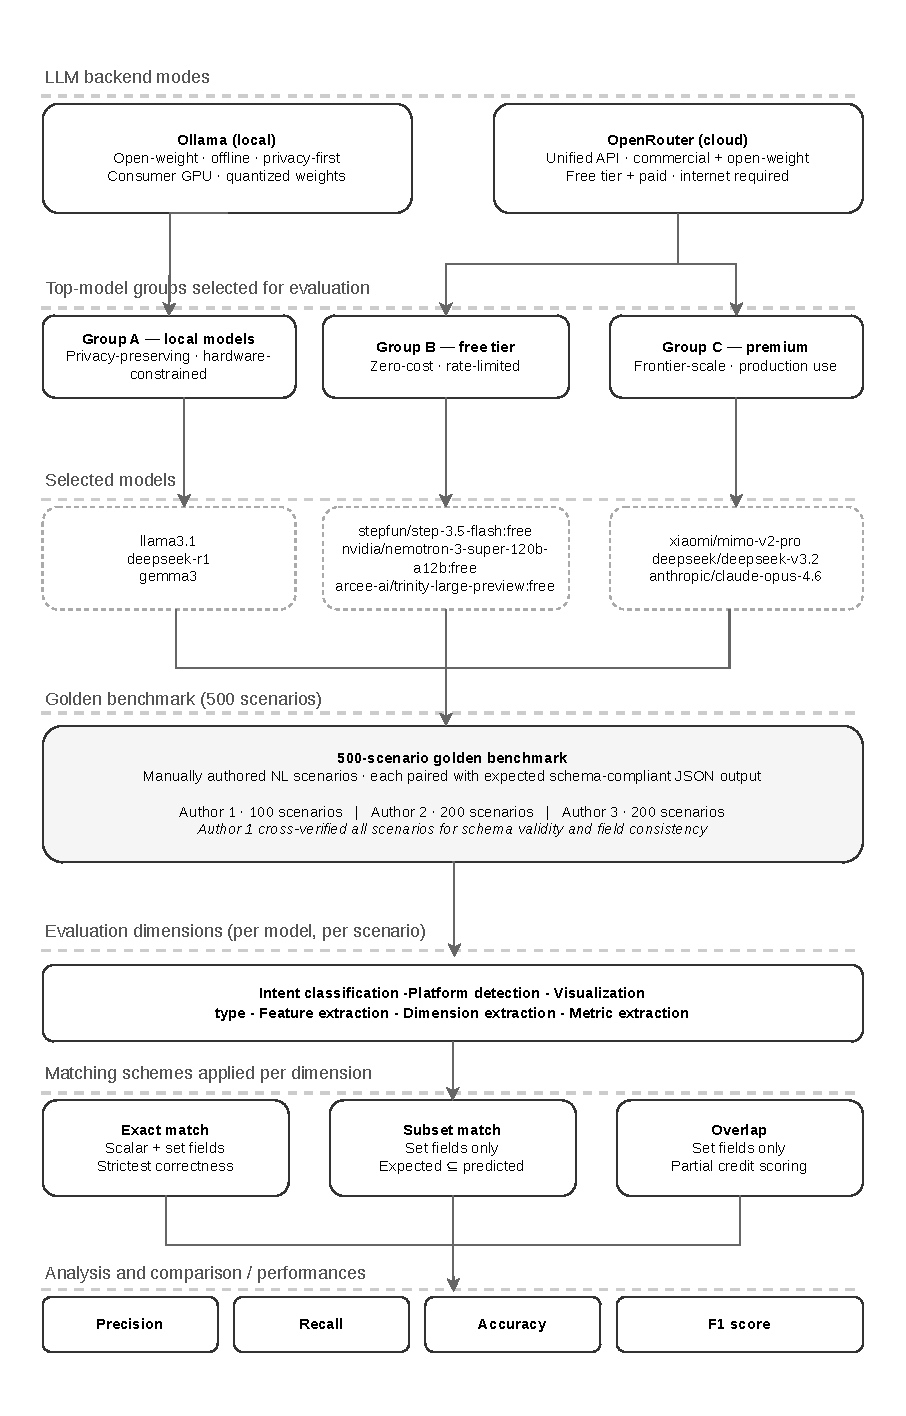
\includegraphics[width=\textwidth]{assets/evaluation_framework.pdf}
    \caption{Vue d'ensemble du cadre d'évaluation de la couche LLM de RevMine}
    \label{fig:eval-framework}
\end{figure}

L'évaluation porte sur six \textbf{dimensions}, chacune correspondant à un champ du schéma JSON
et à un mode de défaillance identifié lors de l'ingénierie des prompts.

\begin{table}[H]
\centering
\small
\caption{Dimensions d'évaluation de la couche LLM et impact opérationnel des erreurs}
\label{tab:eval_dim_fr}
\begin{tabular}{|>{\raggedright\arraybackslash}p{3.5cm}
                |>{\centering\arraybackslash}p{1.8cm}
                |>{\raggedright\arraybackslash}p{7cm}|}
\hline
\textbf{Dimension (champ JSON)} & \textbf{Type} & \textbf{Impact en cas d'erreur} \\
\hline
Intention (\texttt{intent}) & Scalaire & Critique~: mauvais pipeline déclenché \\
\hline
Plateforme (\texttt{platform}) & Scalaire & Élevé~: appels API vers la mauvaise source \\
\hline
Visualisation (\texttt{visualization}) & Scalaire & Moyen~: graphique inadapté \\
\hline
Métriques (\texttt{metrics}) & Ensemble & Critique~: lacunes silencieuses ou noms rejetés \\
\hline
Features (\texttt{features}) & Ensemble & Élevé~: colonnes absentes du dataset de sortie \\
\hline
Dimensions analytiques (\texttt{dimensions}) & Ensemble & Moyen~: agrégations incohérentes \\
\hline
\end{tabular}
\end{table}

Les champs scalaires sont évalués par \textbf{correspondance exacte}. Les champs ensemblistes sont
évalués selon trois critères~: correspondance exacte (ensemble prédit identique à l'ensemble
attendu), correspondance par sous-ensemble (tous les éléments attendus sont présents), et métriques
de recouvrement (précision, rappel, F\textsubscript{1}).

\subsubsection{Modèles évalués}

Neuf modèles ont été évalués, organisés en trois groupes reflétant les principaux contextes de
déploiement de RevMine~: modèles locaux via Ollama (Groupe~A), modèles hébergés gratuits via
OpenRouter (Groupe~B) et modèles premium via OpenRouter (Groupe~C).

\begin{table}[H]
\centering
\small
\caption{Correspondance des abréviations des modèles évalués}
\label{tab:rq2_abbrev_fr}
\begin{tabular}{|>{\raggedright\arraybackslash}p{4cm}
                |>{\raggedright\arraybackslash}p{9cm}|}
\hline
\textbf{Abréviation} & \textbf{Identifiant complet} \\
\hline
\texttt{llama-3.1-8b}    & \texttt{meta-llama/llama-3.1-8b-instruct} \\
\hline
\texttt{gemma-3-27b}     & \texttt{google/gemma-3-27b-it} \\
\hline
\texttt{deepseek-r1}     & \texttt{deepseek/deepseek-r1} \\
\hline
\texttt{step-3.5-flash}  & \texttt{stepfun/step-3.5-flash:free} \\
\hline
\texttt{nemotron-120b}   & \texttt{nvidia/nemotron-3-super-120b-a12b:free} \\
\hline
\texttt{trinity-large}   & \texttt{arcee-ai/trinity-large-preview:free} \\
\hline
\texttt{claude-opus-4.6} & \texttt{anthropic/claude-opus-4.6} \\
\hline
\texttt{mimo-v2-pro}     & \texttt{xiaomi/mimo-v2-pro} \\
\hline
\texttt{deepseek-v3.2}   & \texttt{deepseek/deepseek-v3.2} \\
\hline
\end{tabular}
\end{table}

\subsection{Résultats~: dimensions scalaires et conformité au schéma}

\begin{table}[H]
\centering
\small
\caption{RQ2 -- Validité du pipeline et dimensions scalaires}
\label{tab:rq2_scalar_fr}
\begin{tabular}{|>{\centering\arraybackslash}p{0.8cm}
                |>{\raggedright\arraybackslash}p{3.8cm}
                |>{\centering\arraybackslash}p{1.5cm}
                |>{\centering\arraybackslash}p{1.5cm}
                |>{\centering\arraybackslash}p{1.5cm}
                |>{\centering\arraybackslash}p{1.7cm}
                |>{\centering\arraybackslash}p{1.7cm}|}
\hline
\textbf{Grp} & \textbf{Modèle} & \textbf{Taux succès} & \textbf{JSON valide} & \textbf{EM total} & \textbf{Acc. intention} & \textbf{Acc. plateforme} \\
\hline
\multicolumn{7}{|l|}{\textit{Groupe A -- local (Ollama)}} \\
\hline
A & \texttt{llama-3.1-8b}    & 0,960 & 0,960 & 0,010 & 0,928 & 0,763 \\
A & \texttt{gemma-3-27b}     & 0,955 & 0,955 & 0,198 & 0,900 & 0,882 \\
A & \texttt{deepseek-r1}     & 0,963 & 0,963 & 0,238 & 0,948 & 0,844 \\
\hline
\multicolumn{7}{|l|}{\textit{Groupe B -- gratuit (OpenRouter)}} \\
\hline
B & \texttt{step-3.5-flash}  & 0,943 & 0,943 & 0,250 & 0,765 & 0,696 \\
B & \texttt{nemotron-120b}   & 0,920 & 0,920 & 0,270 & 0,908 & 0,726 \\
B & \texttt{trinity-large}   & 0,995 & 0,995 & 0,265 & 0,973 & 0,889 \\
\hline
\multicolumn{7}{|l|}{\textit{Groupe C -- premium (OpenRouter)}} \\
\hline
C & \texttt{claude-opus-4.6} & 0,988 & 0,988 & 0,268 & 0,978 & 0,911 \\
C & \texttt{mimo-v2-pro}     & 0,995 & 0,995 & 0,255 & 0,988 & 0,896 \\
C & \texttt{deepseek-v3.2}   & 0,963 & 0,963 & 0,183 & 0,940 & 0,882 \\
\hline
\end{tabular}
\end{table}

La conformité au schéma est élevée sur tous les modèles (taux de succès entre 92,0\,\% et
99,5\,\%). En revanche, la correspondance exacte globale -- qui exige que chaque champ du schéma
soit simultanément correct -- est nettement plus faible, de 1,0\,\% à 27,0\,\%. Ce contraste
montre que la principale difficulté dans RevMine n'est pas de générer un objet JSON bien formé,
mais de produire un objet sémantiquement correct sur l'ensemble des champs requis.

La classification de l'intention est la dimension scalaire la plus fiable, avec les meilleurs
modèles approchant les performances plafonds (\texttt{mimo-v2-pro} à 98,8\,\%,
\texttt{claude-opus-4.6} à 97,8\,\%, \texttt{trinity-large} à 97,3\,\%). La détection de la
plateforme (entre 69,6\,\% et 91,1\,\%) et la sélection de la visualisation restent plus
sujettes aux erreurs, notamment pour les modèles gratuits.

\subsection{Résultats~: dimensions ensemblistes}

\begin{table}[H]
\centering
\small
\caption{RQ2 -- Dimensions ensemblistes (correspondance exacte, sous-ensemble et recouvrement)}
\label{tab:rq2_set_fr}
\begin{tabular}{|>{\centering\arraybackslash}p{0.6cm}
                |>{\raggedright\arraybackslash}p{3.6cm}
                |>{\centering\arraybackslash}p{0.9cm}
                |>{\centering\arraybackslash}p{0.9cm}
                |>{\centering\arraybackslash}p{0.9cm}
                |>{\centering\arraybackslash}p{0.9cm}
                |>{\centering\arraybackslash}p{0.9cm}
                |>{\centering\arraybackslash}p{0.9cm}
                |>{\centering\arraybackslash}p{0.9cm}
                |>{\centering\arraybackslash}p{0.9cm}
                |>{\centering\arraybackslash}p{0.9cm}|}
\hline
 & & \multicolumn{3}{c|}{\textbf{Features}} & \multicolumn{3}{c|}{\textbf{Dimensions}} & \multicolumn{3}{c|}{\textbf{Métriques}} \\
\hline
\textbf{Grp} & \textbf{Modèle} & EM & Sub & F1 & EM & Sub & F1 & EM & Sub & F1 \\
\hline
\multicolumn{11}{|l|}{\textit{Groupe A -- local (Ollama)}} \\
\hline
A & \texttt{llama-3.1-8b}    & 0,775 & 0,787 & 0,202 & 0,497 & 1,000 & 0,000 & 0,393 & 0,648 & 0,706 \\
A & \texttt{gemma-3-27b}     & 0,889 & 0,919 & 0,340 & 0,958 & 1,000 & 0,000 & 0,378 & 0,618 & 0,687 \\
A & \texttt{deepseek-r1}     & 0,898 & 0,902 & 0,315 & 0,976 & 1,000 & 0,000 & 0,455 & 0,705 & 0,780 \\
\hline
\multicolumn{11}{|l|}{\textit{Groupe B -- gratuit (OpenRouter)}} \\
\hline
B & \texttt{step-3.5-flash}  & 0,847 & 0,885 & 0,297 & 0,958 & 1,000 & 0,000 & 0,448 & 0,725 & 0,749 \\
B & \texttt{nemotron-120b}   & 0,855 & 0,860 & 0,266 & 0,988 & 1,000 & 0,000 & 0,465 & 0,663 & 0,756 \\
B & \texttt{trinity-large}   & 0,821 & 0,953 & 0,335 & 0,927 & 1,000 & 0,000 & 0,460 & 0,763 & 0,739 \\
\hline
\multicolumn{11}{|l|}{\textit{Groupe C -- premium (OpenRouter)}} \\
\hline
C & \texttt{claude-opus-4.6} & 0,570 & 0,953 & 0,310 & 0,927 & 1,000 & 0,000 & 0,430 & 0,873 & 0,776 \\
C & \texttt{mimo-v2-pro}     & 0,851 & 0,949 & 0,336 & 0,897 & 1,000 & 0,000 & 0,475 & 0,815 & 0,821 \\
C & \texttt{deepseek-v3.2}   & 0,855 & 0,945 & 0,326 & 0,891 & 1,000 & 0,000 & 0,433 & 0,820 & 0,738 \\
\hline
\end{tabular}
\end{table}

Les valeurs de correspondance par sous-ensemble pour les dimensions ensemblistes sont nettement
supérieures aux valeurs de correspondance exacte. Pour l'extraction de métriques,
\texttt{claude-opus-4.6} passe de 43,0\,\% en exact match à 87,3\,\% en sous-ensemble, et
\texttt{mimo-v2-pro} de 47,5\,\% à 81,5\,\%, montrant que les modèles récupèrent généralement
les informations requises accompagnées d'éléments supplémentaires plutôt qu'ils ne les omettent.
Le F\textsubscript{1} de recouvrement sur l'extraction de métriques est fort pour les modèles
leaders (\texttt{mimo-v2-pro}~: 0,821~; \texttt{deepseek-r1}~: 0,780~;
\texttt{claude-opus-4.6}~: 0,776), tandis que l'extraction de features est sensiblement plus
faible (0,202 à 0,340), indiquant que les omissions et sur-prédictions sur les features dérivées
sont plus fréquentes.

\subsection{Résultats~: complétude des dépendances features-métriques}
\label{subsec:rq3-resultats}

\subsubsection{Enjeux et mesures}

Cette analyse approfondit la question de la correction exécutable en examinant la capacité des
modèles à inférer l'ensemble des métriques brutes requises par les features calculées
demandées. Une dépendance manquante produit un \textbf{échec silencieux}~: la collecte se
termine, le CSV est produit, aucune erreur n'est levée, mais la colonne dérivée demandée est
absente du dataset, car les champs bruts nécessaires à son calcul n'ont jamais été récupérés.
Contrairement à l'hallucination d'une métrique -- rejetée immédiatement par le service de
collecte -- l'omission d'une dépendance n'est détectable qu'à l'inspection du dataset résultant,
rendant ces défaillances particulièrement néfastes pour la reproductibilité.

Deux métriques complémentaires ont été définies. Le \textbf{Rappel de Dépendances de Feature}
(\textit{Feature Dependency Recall}, FDR) mesure la proportion de métriques brutes requises pour
une feature donnée effectivement incluses dans la sortie du modèle, moyennée sur toutes les
features du scénario~:

\begin{equation}
\mathrm{FDR}(s) = \frac{1}{|F_s|} \sum_{f \in F_s}
\frac{|\mathrm{deps}(f) \cap \hat{M}_s|}{|\mathrm{deps}(f)|}
\end{equation}

Le \textbf{Taux de Satisfaction Complète des Dépendances} (\textit{Full Dependency Satisfaction
Rate}, FDSR) est la proportion de scénarios comportant des features pour lesquels toutes les
métriques brutes requises de toutes les features demandées sont présentes dans la sortie~:

\begin{equation}
\mathrm{FDSR} = \frac{|\{ s \in S_F \mid \forall f \in F_s :
\mathrm{deps}(f) \subseteq \hat{M}_s \}|}{|S_F|}
\end{equation}

Le FDSR est la métrique principale~: un seul dépendance manquante sur une seule feature constitue
un échec complet du scénario, car la colonne associée sera silencieusement absente du CSV de
sortie. Le FDR est rapporté comme diagnostic secondaire pour caractériser les patterns d'échecs
partiels.

\subsubsection{Résultats et implications}

Le FDSR strict reste bien en dessous du seuil de succès de 90\,\% pour tous les modèles évalués,
tandis que les valeurs de FDR sont substantiellement plus élevées -- indiquant que, lorsqu'un
modèle échoue sur un scénario, il manque généralement une seule dépendance plutôt que plusieurs.
Ce pattern est cohérent avec les résultats de correspondance exacte sur les métriques observés
(37,8\,\%--47,5\,\%)~: une seule dépendance manquante suffit à faire échouer entièrement un
scénario sous FDSR. Il est également cohérent avec les valeurs élevées de rappel observées pour
l'extraction de métriques (0,739 à 0,941 pour le champ ensembliste \texttt{metrics}), montrant
que les modèles récupèrent généralement la majorité des métriques requises mais en omettent
occasionnellement une ou deux.

La mitigation naturelle pour les échecs FDSR est \textbf{architecturale plutôt qu'au niveau du
modèle}~: puisque RevMine connaît de manière déterministe la table de dépendances depuis son
propre service d'analyse, l'injection automatique de toute dépendance manquante avant l'exécution
du plan de collecte fait monter le FDSR effectif à 100\,\% par construction. Avec cette
mitigation architecturale en place, le modèle est responsable de l'identification des features
demandées par l'utilisateur, tandis que la clôture des dépendances est assurée par le pipeline
lui-même -- permettant ainsi d'utiliser la couche d'orchestration dans un contexte pleinement
automatisé même aux niveaux de performance actuels des modèles.

% ============================================================

\section{Menaces à la validité}
\label{sec:menaces-validite}

\subsection{Validité interne}

Le principal risque interne est la dépendance entre RevMine et l'oracle. Pour limiter ce risque, l'oracle doit être implémenté indépendamment, avec des fonctions simples et auditables, et ne doit pas importer les modules du service d'analyse RevMine.

\subsection{Validité externe}

Le corpus de validation peut ne pas représenter tous les types de dépôts open source ou industriels. Il faut donc diversifier les tailles de projets, les plateformes, les langages et les pratiques de revue. Les conclusions doivent être formulées comme valides pour le corpus étudié et non comme une preuve universelle.

\subsection{Validité de construction}

Certaines métriques peuvent avoir plusieurs définitions acceptables. Par exemple, le review time peut être défini comme le temps jusqu'au premier commentaire, jusqu'à la première revue formelle ou jusqu'à l'approbation. Le rapport doit donc fixer explicitement la définition utilisée par RevMine avant d'interpréter les résultats.

\subsection{Validité de conclusion}

Les seuils d'acceptation doivent être définis avant l'analyse. Les résultats incomplets, les écarts liés à des limitations d'API et les cas non couverts doivent être rapportés explicitement afin d'éviter une interprétation excessive des performances.

\section{Conclusion}
\label{sec:conclusion-validation}

Ce chapitre propose une validation plus complète et plus défendable de RevMine. Les tests automatisés démontrent la robustesse logicielle, la validation de collecte vérifie la parité avec un collecteur de référence, l'évaluation LLM mesure la capacité de traduction du langage naturel vers des plans structurés, et la validation calculatoire ajoutée vérifie la contribution centrale de la plateforme : produire des métriques et des analyses correctes à partir de données de revue de code.

La méthode la plus importante à intégrer est la validation par oracle indépendant. Elle permet de transformer la validation de RevMine en une démarche mesurable, reproductible et scientifiquement défendable. Après exécution du protocole, les tableaux de résultats devront être complétés avec les valeurs observées et les éventuels écarts devront être discutés comme limites documentées plutôt que masqués.
